% Options for packages loaded elsewhere
\PassOptionsToPackage{unicode}{hyperref}
\PassOptionsToPackage{hyphens}{url}
\PassOptionsToPackage{dvipsnames,svgnames,x11names}{xcolor}
%
\documentclass[
  letterpaper,
]{tex/svmono}

\usepackage{amsmath,amssymb}
\usepackage{iftex}
\ifPDFTeX
  \usepackage[T1]{fontenc}
  \usepackage[utf8]{inputenc}
  \usepackage{textcomp} % provide euro and other symbols
\else % if luatex or xetex
  \usepackage{unicode-math}
  \defaultfontfeatures{Scale=MatchLowercase}
  \defaultfontfeatures[\rmfamily]{Ligatures=TeX,Scale=1}
\fi
\usepackage{lmodern}
\ifPDFTeX\else  
    % xetex/luatex font selection
\fi
% Use upquote if available, for straight quotes in verbatim environments
\IfFileExists{upquote.sty}{\usepackage{upquote}}{}
\IfFileExists{microtype.sty}{% use microtype if available
  \usepackage[]{microtype}
  \UseMicrotypeSet[protrusion]{basicmath} % disable protrusion for tt fonts
}{}
\makeatletter
\@ifundefined{KOMAClassName}{% if non-KOMA class
  \IfFileExists{parskip.sty}{%
    \usepackage{parskip}
  }{% else
    \setlength{\parindent}{0pt}
    \setlength{\parskip}{6pt plus 2pt minus 1pt}}
}{% if KOMA class
  \KOMAoptions{parskip=half}}
\makeatother
\usepackage{xcolor}
\setlength{\emergencystretch}{3em} % prevent overfull lines
\setcounter{secnumdepth}{5}
% Make \paragraph and \subparagraph free-standing
\ifx\paragraph\undefined\else
  \let\oldparagraph\paragraph
  \renewcommand{\paragraph}[1]{\oldparagraph{#1}\mbox{}}
\fi
\ifx\subparagraph\undefined\else
  \let\oldsubparagraph\subparagraph
  \renewcommand{\subparagraph}[1]{\oldsubparagraph{#1}\mbox{}}
\fi


\providecommand{\tightlist}{%
  \setlength{\itemsep}{0pt}\setlength{\parskip}{0pt}}\usepackage{longtable,booktabs,array}
\usepackage{calc} % for calculating minipage widths
% Correct order of tables after \paragraph or \subparagraph
\usepackage{etoolbox}
\makeatletter
\patchcmd\longtable{\par}{\if@noskipsec\mbox{}\fi\par}{}{}
\makeatother
% Allow footnotes in longtable head/foot
\IfFileExists{footnotehyper.sty}{\usepackage{footnotehyper}}{\usepackage{footnote}}
\makesavenoteenv{longtable}
\usepackage{graphicx}
\makeatletter
\def\maxwidth{\ifdim\Gin@nat@width>\linewidth\linewidth\else\Gin@nat@width\fi}
\def\maxheight{\ifdim\Gin@nat@height>\textheight\textheight\else\Gin@nat@height\fi}
\makeatother
% Scale images if necessary, so that they will not overflow the page
% margins by default, and it is still possible to overwrite the defaults
% using explicit options in \includegraphics[width, height, ...]{}
\setkeys{Gin}{width=\maxwidth,height=\maxheight,keepaspectratio}
% Set default figure placement to htbp
\makeatletter
\def\fps@figure{htbp}
\makeatother

\usepackage{booktabs}

\usepackage{float}
\usepackage{index}
% index functions separately
\newindex{code}{adx}{and}{R code index}
\newcommand{\indexf}[1]{\index[code]{#1@\texttt{#1()}}}
\newcommand{\indexc}[1]{\index[code]{#1@\texttt{#1}}}

\DeclareGraphicsExtensions{.pdf,.png}

\usepackage{hyperref}
% Place links in parens
\renewcommand{\href}[2]{#2 (\url{#1})}
% Use auto ref for internal links
\let\oldhyperlink=\hyperlink
\renewcommand{\hyperlink}[2]{\autoref{#1}}
\def\chapterautorefname{Chapter}
\def\sectionautorefname{Section}
\def\subsectionautorefname{Section}
\def\subsubsectionautorefname{Section}

\setlength{\emergencystretch}{3em}  % prevent overfull lines
\vbadness=10000 % suppress underfull \vbox
\hbadness=10000 % suppress underfull \vbox
\hfuzz=10pt

\makeindex
\makeatletter
\makeatother
\makeatletter
\@ifpackageloaded{bookmark}{}{\usepackage{bookmark}}
\makeatother
\makeatletter
\@ifpackageloaded{caption}{}{\usepackage{caption}}
\AtBeginDocument{%
\ifdefined\contentsname
  \renewcommand*\contentsname{Table of contents}
\else
  \newcommand\contentsname{Table of contents}
\fi
\ifdefined\listfigurename
  \renewcommand*\listfigurename{List of Figures}
\else
  \newcommand\listfigurename{List of Figures}
\fi
\ifdefined\listtablename
  \renewcommand*\listtablename{List of Tables}
\else
  \newcommand\listtablename{List of Tables}
\fi
\ifdefined\figurename
  \renewcommand*\figurename{Figure}
\else
  \newcommand\figurename{Figure}
\fi
\ifdefined\tablename
  \renewcommand*\tablename{Table}
\else
  \newcommand\tablename{Table}
\fi
}
\@ifpackageloaded{float}{}{\usepackage{float}}
\floatstyle{ruled}
\@ifundefined{c@chapter}{\newfloat{codelisting}{h}{lop}}{\newfloat{codelisting}{h}{lop}[chapter]}
\floatname{codelisting}{Listing}
\newcommand*\listoflistings{\listof{codelisting}{List of Listings}}
\makeatother
\makeatletter
\@ifpackageloaded{caption}{}{\usepackage{caption}}
\@ifpackageloaded{subcaption}{}{\usepackage{subcaption}}
\makeatother
\makeatletter
\@ifpackageloaded{tcolorbox}{}{\usepackage[skins,breakable]{tcolorbox}}
\makeatother
\makeatletter
\@ifundefined{shadecolor}{\definecolor{shadecolor}{rgb}{.97, .97, .97}}
\makeatother
\makeatletter
\makeatother
\makeatletter
\makeatother
\ifLuaTeX
  \usepackage{selnolig}  % disable illegal ligatures
\fi
\usepackage[]{natbib}
\bibliographystyle{plainnat}
\IfFileExists{bookmark.sty}{\usepackage{bookmark}}{\usepackage{hyperref}}
\IfFileExists{xurl.sty}{\usepackage{xurl}}{} % add URL line breaks if available
\urlstyle{same} % disable monospaced font for URLs
\hypersetup{
  pdftitle={Credit Scoring},
  pdfauthor={Juan Isaula},
  colorlinks=true,
  linkcolor={blue},
  filecolor={Maroon},
  citecolor={Blue},
  urlcolor={Blue},
  pdfcreator={LaTeX via pandoc}}

\title{Credit Scoring}
\author{Juan Isaula}
\date{}

\begin{document}
\maketitle
\null\vfill
\begin{flushleft}
\thispagestyle{empty}
\textit{R for Clinical Study Reports and Submission}

© Placeholder Name, Inc.

ISBN-1234567891234

\noindent Lorem ipsum dolor sit amet, consectetur adipiscing elit.
Nulla et elementum libero. In hac habitasse platea dictumst.
Vestibulum ante ipsum primis in faucibus orci luctus et ultrices
posuere cubilia Curae; Donec sed odio dui. Nullam quis risus eget
urna mollis ornare vel eu leo. Pellentesque habitant morbi tristique
senectus et netus et malesuada fames ac turpis egestas.
Curabitur blandit tempus porttitor.
Integer posuere erat a ante venenatis dapibus posuere velit aliquet.
\end{flushleft}

\frontmatter

% Dedication
\begin{center}
    \thispagestyle{empty}
    \vspace*{\fill}
    \huge{\textit{Placeholder for dedication text}}
    \vspace*{\fill}
\end{center}

\mainmatter

\ifdefined\Shaded\renewenvironment{Shaded}{\begin{tcolorbox}[interior hidden, sharp corners, enhanced, frame hidden, boxrule=0pt, borderline west={3pt}{0pt}{shadecolor}, breakable]}{\end{tcolorbox}}\fi

\renewcommand*\contentsname{Table of contents}
{
\hypersetup{linkcolor=}
\setcounter{tocdepth}{2}
\tableofcontents
}
\bookmarksetup{startatroot}

\hypertarget{welcome}{%
\chapter*{Welcome}\label{welcome}}
\addcontentsline{toc}{chapter}{Welcome}

\markboth{Welcome}{Welcome}

Bienvenidos, en este artículo te presento algunos modelos tradicionales,
modernos y conceptos fundamentales para que te encamines al mundo del
\emph{Credit Scoring.} Existen algunas definiciones para Credit Scoring;
sin embargo, en este trabajo, se considera a un credit scoring como un
conjunto de metodologías que permitan evidenciar la probabilidad que un
cliente cumpla o no con sus obligaciones, a partir de la información que
se conozca del mismo. Estos modelos tienen muchas funciones dentro del
ciclo de vida de un crédito que comprende el otorgamiento, seguimiento,
cobranza y recuperación; sin embargo, este artículo se enfocará en las
metodologías que sirven de apoyo, en la toma de decisiones del proceso
de otorgamiento de créditos; tales metodologías deben permitir medir los
riesgos de los potenciales clientes, a fin de precisar quienen podrían
ser sujetos de crédito, estableciendo variables significativas que
ayudan a identificar los individuos cuyo riesgo se ajuste al perfil de
riesgo de la institución.

Welcome, in this article we present some traditional and modern models
and fundamental concepts to guide you into the world of Credit Scoring.
There are a few definitions for Credit Scoring; However, in this work,
credit scoring is considereded as a set of methodologies that allow us
to demonstrate the probability that a client meets or does not comply
with its obligations, based on the information known about it. These
models have many functions within the life cycle of a loan that includes
granting, monitoring, collection and recovery; However, this article
will focus on the methodologies that serve as support in decision making
in the credit granting process; such methodologies must allow measuring
the risks of potential clients, in order to specify who could be subject
to credit, establishing significant variables that help identify
individuals whose risk fits the institution's risk profile.

\bookmarksetup{startatroot}

\hypertarget{preface}{%
\chapter*{Preface}\label{preface}}
\addcontentsline{toc}{chapter}{Preface}

\markboth{Preface}{Preface}

\hypertarget{section}{%
\section*{}\label{section}}
\addcontentsline{toc}{section}{}

\markright{}

En el proceso de otorgamiento de créditos, una institución no puede
tomar decisiones a partir de su juicio de experto para cada una de las
solicitudes recibidas, pues con el aumento en el número de solicitantes
y la competencia intensa en la industria crediticia, este método no
puede satisfacer las demandas en los aspectos economicos y de eficiencia
\citep{Yu}; sino que intentará adoptar sistemas de calificación de
créditos para facilitar y acelerar los procesos en la toma de
decisiones. Por tal motivo, nace el concepto de modelos de
\textbf{\emph{Credit Scoring}} o modelos de calificación de créditos
\citep{Islam}.

Muchos algoritmos son usados para la construcción de un credit scoring,
sin embargo, cada vez se deberá buscar alternativas más efectivas para
tomar decisiones más precisas, por ejemplo, las redes neuronales
\citep{Islam}.

Son muchos los factores que pueden incidir en el crecimiento de la
cartera vencida o el incremento de la mora de una cartera, como malas
prácticas en la concesión de créditos, metas de crédito agresivas por
parte de la institución, deterioro del empleo, recesión ecónomica, etc.
Sin embargo, el anterior escenario evidencia la necesidad de contar con
nuevas herramientas para la gestión de riesgo de crédito que ayuden a
minimizar la probabilidad de pérdida de una institución, buscando
alcanzar la eficiencia de la gestión de riesgos a partir de mejores
herramientas estadísticas e informáticas.

\hypertarget{modelos-credit-scoring}{%
\section*{Modelos Credit Scoring}\label{modelos-credit-scoring}}
\addcontentsline{toc}{section}{Modelos Credit Scoring}

\markright{Modelos Credit Scoring}

Los modelos credit Scoring son algoritmos o métodos que pueden ayudar a
obtener la probabilidad de incumplimiento de un solicitante de crédito,
permitiendo evaluar el riesgo en el origen de la financiación
\citep{Gutierrez}.

\bookmarksetup{startatroot}

\hypertarget{modelos-credit-scoring-1}{%
\chapter{Modelos Credit Scoring}\label{modelos-credit-scoring-1}}

Los modelos credit Scoring son algoritmos o métodos que pueden ayudar a
obtener la probabilidad de incumplimiento de un solicitante de crédito,
permitiendo evaluar el riesgo en el origen de la financiación
\citep{Gutierrez}.

El objetivo principal de estos modelos es estimar la probabilidad de
incumplimiento de un solicitante de crédito; para esto es necesario
contar con una variable que identifique si el solicitante es un buen o
mal cliente, esta variable será represantada con la letra
\(\textbf{Y}\), que es la variable dependiente del modelo.

La variable dependiente es una variable dicotómica (binaria) que toma
los siguientes valores:

\[
Y = \left \{
\begin{array}{rr}
1 &: \mbox{Si el solicitante de crédito es definido como un buen cliente}\\
0 &: \mbox{Si el solicitante de crédito es definido como un mal cliente}\\
\end{array}
\right. \hspace{1.5cm} (1)
\]

La definición para la variable dependiente \(\textbf{Y}\), es construida
a partir de información demográfica, comportamiento en el buró y/o
dentro de la institución.

Los modelos buscan estimar la probabilidad que la variable dependiente
\(\textbf{Y}\) tome el valor de 0 o 1, a partir de un conjunto de
variables denominadas independientes, las cuales serán representadas con
la letra \(\textbf{X}\), que puede ser cualitativas o cuantitativas. Las
variables independientes son obtenidas a partir de diversas fuentes de
información crediticia, buró, demográfica, etc. Muchas de las cuales
dependerán de las características del crédito que se esté considerando.

\hypertarget{modelo-de-regresiuxf3n-loguxedstica---logit}{%
\section{Modelo de Regresión Logística -
Logit}\label{modelo-de-regresiuxf3n-loguxedstica---logit}}

Los modelos logit pertenecen al grupo jde modelos de regresión con
respuesta cualitativa, en este caso binaria; mientras que las variables
independientes pueden ser cualitativas o cuantitativas, o una mezcla de
ambas \citep{Flórez}.

El modelo está basado en una función de distribución logística, cuya
estructura se presenta a continuación:

\[
P(Y = 1 | X) = F(\textbf{Z}) = \frac{e^{\textbf{Z}}}{1 + e^{\textbf{Z}}}, \hspace{1cm} -\infty < z <\infty,\hspace{1cm} (2)
\]

con
\(z = \textbf{X}^T\beta = \beta_0 + \beta_1x_1 + . . . + \beta_nx_n\).

\begin{figure}

{\centering 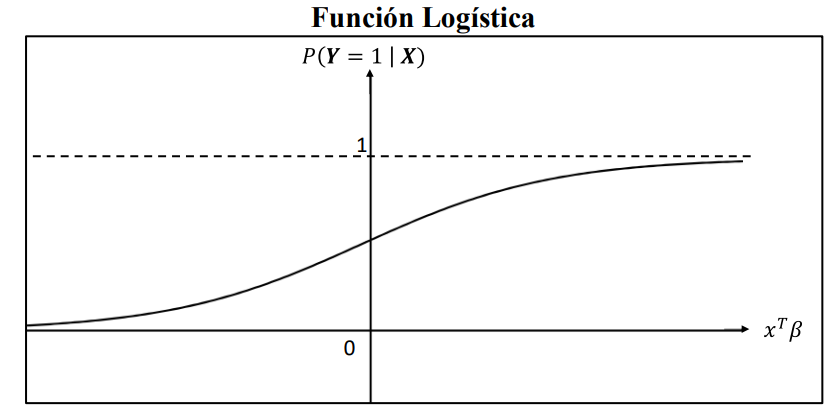
\includegraphics{images/Figura_1.png}

}

\caption{Fuente: Flores y Rincón (2002, 128)}

\end{figure}

donde:

\begin{itemize}
\item
  \$ \textbf{Y:}\$ Es la variable dependiente, binaria, que no puede
  tomar dos posibles valores, que se etiquetarán con 0 (cliente malo) y
  1 (cliente bueno).
\item
  \(\textbf{X:}\) Es el conjunto de \(n\) variables independientes
  \((x_1, x_2, . . . , x_n)\) relacionadas con la información propia del
  solicitante, tomadas con el fin de explicar y/o predecir el valor de
  \(\textbf{Y}\).
\item
  \(F(\textbf{Z}):\) Es la función de probabilidad, que depende de un
  vector de parámetros \(\beta = (\beta_0, \beta_1, . . . , \beta_n)\),
  que permitirán relacionar las variables independientes \(\textbf{X}\),
  con la dependiente \(\textbf{Y}\). Esta función tiene un rango entre
  \([0,1]\) y se conoce como función de distribución logística.
\item
  El objetivo del modelo es encontrar los coeficientes \(\beta\) que
  mejor se ajustan a la expresión \(P(Y = 1|X)\).
\end{itemize}

\hypertarget{estimaciuxf3n-de-los-paruxe1metros-del-modelo-logit}{%
\subsection{Estimación de los parámetros del modelo
logit}\label{estimaciuxf3n-de-los-paruxe1metros-del-modelo-logit}}

La estimación de los coeficientes \(\beta\) puede realizarse a partir
del método de máxima verosimilitud \citep{Guajarati}.

Supóngase que se cuenta con un conjunto de \(k\) individuos; de tal
forma que, catalogarles como buenos o malos clientes será definido por
la variable \(Y_i\), considerando \(i = 1, . . . , k\).

En vista que cada \(Y_i\) es una variable aleatoria de Bernoulli, por
tomar dos valores, 0 o 1, podemos expresar la probabilidad que suceda
uno u otro evento, como sigue:

\[
\begin{eqnarray}
P(Y_i = 1) &=& P_i\\[0.2cm]
P(Y_i = 0) &=& 1 - P_i 
\end{eqnarray}
\]

su función de probabilidad será:

\[
f_i(Y_i) = P_i^{Y_i}\times (1 - P_i)^{1-Y_i}, \hspace{1cm} i = 1, . . . , k\hspace{1cm} (3)
\]

Es decir, la función \(f_i(Y_i)\) denota la probabilidad de
\(Y_i = 0~ o~ 1\).

Como cada observación es independiente, la probabilidad conjunta de
observar los \(k\) valores de la variable \(Y\), se expresa como:

\[
f(Y_1, Y_2, . . . , Y_k) = \prod_{i=1}^{k} f_i(Y_i) = \prod_{i=1}^{k} P_i^{Y_i}
\times (1- P_i)^{1-Y_i}\hspace{1cm}(4)\]

A está probabilidad conjunta se le conoce como \textbf{\emph{función de
verosimilitud}}. Al tomar el logaritmo de está función se tiene:

\[
\begin{eqnarray}
\ln(f(Y_1, Y_2, . . . , Y_k)) &=& \left[Y_i\ln P_i + (1 - P_i)\ln(1 - P_i)\right]\\[0.2cm]
&=& \sum_{i=1}^{k} \left[Y_i\ln P_i - Y_i\ln(1-P_i) + \ln(1 - P_i)\right]\\[0.2cm]
&=& \sum_{i=1}^{k} \left[Y_i\ln\left(\frac{P_i}{1 - P_i}\right)\right] + \sum_{i=1}^{k}\ln(1 - P_i)\hspace{1.5cm} (5)
\end{eqnarray}
\]

Tal como se expuso en ecuación \((2)\), la probabilidad de que un
individuo sea un buen o mal cliente es representado por:

\[
P_i = \frac{e^{X_i^T\beta}}{1 + e^{X_i^T\beta}} \hspace{1cm} (6)
\]

De aquí se puede, facilmente, demostrar que:

\[
1 - P_i = \frac{1}{1 + e^{X_i^T\beta}}\hspace{1cm}(7)
\]

De igual forma,

\[
\ln\left(\frac{P_i}{1-P_i}\right) = X_i^T\beta\hspace{1cm} (8)
\]

Considerando \((7)\) y \((8)\) en \((5)\) , se puede expresar el
logaritmo de la función de verosimilitud, como sigue

\[
\ln\left(f(Y_1, . . . , Y_k)\right) = \sum_{i=1}^{k}Y_i(X_i^T\beta) - \sum_{i=1}^{k}\ln\left(1 + e^{X_i^T\beta}\right)\hspace{1cm} (9)
\]

Podemos observar que \((9)\) es una función que depende de los
coeficientes \(\beta\), pues \(Y_i\) y \(X_i\) se conocen.

El método de máxima verosimilitud consiste en maximizar la expresión
\((9)\), para buscar la máxima capacidad predictiva. Para esto se deriva
parcialmente, respecto a cada una de las incógnitas; es decir, respecto
a cada \(\beta_j\), con \(j = 1, . . . , n\). Obteniendo un sistema de
\(n\) ecuaciones no lineales, que deberán resolverse por procedimientos
numéricos.

Una vez obtenidos los \(\beta\) se verifica que en verdad maximicen la
función de verosimilitud a partir de la condición de maximización de
segundo orden. Luego de este proceso, se obtiene los coeficientes,
necesarios para estimar la probabilidad de incumplimiento de un
individuo, a partir de la ecuación \((2)\).

\hypertarget{interpretaciuxf3n-coeficientes-de-una-regresiuxf3n-loguxedstica}{%
\subsection{Interpretación coeficientes de una regresión
logística}\label{interpretaciuxf3n-coeficientes-de-una-regresiuxf3n-loguxedstica}}

Una de las razones, por las cuales se utiliza con mayor frecuencia un
modelo de regresión logística es que su interpretación es relativamente
sencilla. Para apreciar este beneficio, es de ayuda entender el
significado de \textbf{\emph{odds}}. Tal como lo expresa \citep{Allison}
muchas personas consideran a una probabilidad como la forma
\emph{natural} de cuantificar que un evento ocurra, considerando valores
que se mueven entre 0 y 1. Sin embargo, existen otras formas de
representar un cambio natural en algún evento, esto son los
\textbf{\emph{odds ratios}}.

El mismo autor, define los \textbf{\emph{odds}}, como la relación entre
el número esperado de veces que un evento ocurra y el número esperado de
veces que este no ocurra. De esta forma, la relación entre el
\textbf{\emph{odds}} y la probabilidad es:

\[
Odds = \frac{probabilidad~que~un~evento~ocurra}{1 - Probabilidad~que~un~evento~ocurra}
\]

Esta expresión tiene relevancia en un modelo de regresión logística,
pues si se considera \((6)\) y \((7)\) se tienen,

\[
\frac{P_i}{1- P_i} = \frac{\frac{e^{X_i^T\beta}}{1 + e^{X_i^T\beta}}}{\frac{1}{1 + e^{X_i^T\beta}}} = e^{X_i^T\beta}\hspace{1cm} (10) 
\]

A esta expresión se la considera como \textbf{\emph{transformación logit
de la probabilidad}} \(P_i\), cuya parte izquierda es una razón de
probabilidades u \emph{odds} \citep{Flórez}. Al considerar el logaritmo
natural en \((10)\) se obtiene el logaritmo de la razón de proabilidades
conocido como logit y es por este término que al modelo de regresión
logística se lo conoce, también, como modelo logit. Así, se llega a la
ecuación \((8)\).

\[
L = \ln\left(\frac{P_i}{1 - P_i}\right) = X_i^T\beta = \beta_0 + \beta_1x_1 + . . . + \beta_nx_n\hspace{1cm}(11)
\]

De esta forma, la interpretación del modelo está dada por la expresión
\textbf{\emph{logit (L)}}; por ejemplo, \(\beta_2\) mide el cambio en
\(L\) ocasionado por un cambio unitario en \(x_2\), suponiendo constante
el resto de variables explicativas \citep{Guajarati}.

La interpretación del modelo también puede darse a partir del
\textbf{\emph{odds ratio,}} la cual es una medida de la magnitud de
asociación entre dos variables; en este caso, cada una de las
independientes con la dependiente. Un \textbf{\emph{odds ratio}} mayor a
1, muestra que existe una relación positiva o directa entre las dos
variables, mientras que un odds ratio menor a 1, establece una relación
negativa o inversa. Cuando el odds ratio es igual a 1, significa que no
existe una relación entre las mismas \citep{Salas}.

El \textbf{\emph{odds ratio}} puede calcularse a partir de la estimación
de los parámetros del modelo

\[
odds~ratio = e^\beta\hspace{1cm}(12)
\]

\bookmarksetup{startatroot}

\hypertarget{references}{%
\chapter*{References}\label{references}}
\addcontentsline{toc}{chapter}{References}

\markboth{References}{References}

\renewcommand{\bibsection}{}
\bibliography{references.bib}




\backmatter

\let\hyperlink=\oldhyperlink % Restore old hyperlink behaviour
\cleardoublepage
\markboth{Index}{Index}
\addcontentsline{toc}{chapter}{Index}
\printindex

\addcontentsline{toc}{chapter}{Code index}
\printindex[code]

\end{document}
